\chapter{Proposed Algorithm} \label{CHAPTER_proposed_algorithm}
In this thesis we are developing an approach dealing with inference of XML schema, which input consists of two components; a set of XML documents and a set of XQuery queries related to the documents. The proposed algorithm introduced in this chapter describes the processing of XQuery queries only and a combination of its output with an existing method of XML schema inference (to produce a complete XML schema) is discussed in the next chapter.

There is an important assumption placed upon the input XQuery queries saying that each query must be syntactically and semantically correct. That means that if a query was evaluated (using a XQuery processor meeting the XQuery specification), the evaluation would not raise any error, neither static nor dynamic. In other words, each query is syntactically correct and it correctly queries the data in the XML documents.

\begin{figure}
\label{FIG_steps_algorithm}
\caption{Steps of the proposed algorithm.}
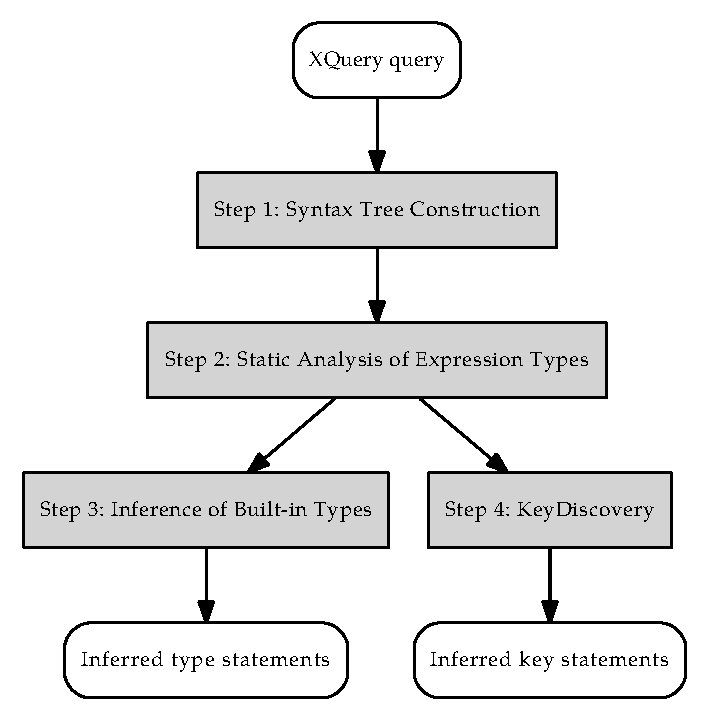
\includegraphics[scale=1]{algorithm.eps}
\end{figure}

The proposed algorithm consists of the following four main steps, show in Figure \ref{FIG_steps_algorithm} and described in detail in the rest of the chapter.

\begin{enumerate}
\item \textbf{Construction of a syntax tree}. We use lexical and syntax analyses proposed in \cite{thesis_schejbal} and for each XQuery on input, we construct a data structure defined in \ref{DEF_syntax_tree}.
\item \textbf{Static Analysis of expression types}. The algorithm searches for expressions in the syntax trees and statically (without evaluation) determines their types.
\item \textbf{Inference of built-in types}. When the types of expressions are determined, selected forms of expression are utilized to infer types of elements and attributes.
\item \textbf{Key discovery}. The final step is an extension of approach \cite{Necasky:2009:DXK:1529282.1529414} inferring keys and foreign keys.
\end{enumerate}

As can be seen in Figure \ref{FIG_steps_algorithm}, step 4 is independent on step 3. They both depend on step 2.

\section{Step 1: Construction of a Syntax Tree}
The first step of the algorithm involves lexical and syntax analyses known from the construction of compilers and produces a so-called syntax tree. The analyses are taken from Ji\v r\'{i} Schejbal's master thesis \cite{thesis_schejbal}. Since they are not directly related to the inference, and thus, they are not directly related to the topic of this thesis, we will not describe them. Nevertheless, they provides us with a helpful processing of XQuery queries and we can focus on the inference.

The syntactic analysis needs to be slightly modified to suit our case. It writes its result into a file in an XML representation. Instead, we need to keep the result in the main memory and pass it to consecutive steps of our algorithm. Though this requirement concerns modifications of implementation, the core of the processing remains untouched. Therefore, we also do not describe these modifications.

\section{Definition of the Syntax Tree}
Firstly, we formally define the syntax tree.

\begin{define}[Syntax tree]
\label{DEF_syntax_tree}
Syntax tree of XQuery query $Q$ is tuple $T = (V, E, c, \mathcal{P}, o)$ where
\begin{itemize}
\item $V \subset \mathbb{N}$ is a set of nodes, each node representing a particular XQuery construct in query $Q$,
\item $E$ is a set of pairs $(v, w)$ where $v,w \in V$ and for every $a, b \in V, a \neq b: (a, b) \in E$ if and only if a construct represented by $b$ is a direct component of a construct represented by $a$ ($b$ is a child of $a$) in query $Q$,
\item $c: V \rightarrow C$ is function assigning each node with its class from set $C$ of all XQuery language constructs listed in Figures \ref{FIG_syntax_tree_node_types_part_1}, \ref{FIG_syntax_tree_node_types_part_2},
\item $\mathcal{P}$ is a set of functions specifying additional properties of the nodes and distinguishing the nodes of the same classes,
\item and $o : V \rightarrow \mathcal{O}$ is a function specifying an order of children of the nodes, where $\mathcal{O} = \{o_v : E_v \rightarrow \mathbb{N} | v \in V, E_v = \{(v, w) | w \in V, (v,w) \in E\}\}$ is set of functions specifying the children order for each node. For every $v \in V, o(v) = o_v$ so that $o_v(v,w)$ is a sequential number of a construct represented by $w$ amongst constructs represented by children of $v$ in query $Q$.
\end{itemize}
\end{define}

Regarding the additional properties, two constructs in $Q$ represented by two nodes of the same class from $C$ may differ in certain ways, and therefore, it is needed to distinguish them. For instance, two different literal values in $Q$ are represented by nodes $l_1, l_2 \in V$ and $c(l_1) = c(l_2) =$ \texttt{LiteralNode} but each has a different value and type. Therefore $\mathcal{P}$ contains functions \\
$type_{LiteralNode}: V_{LiteralNode} \rightarrow Types_{literal}$ \\
$value_{LiteralNode}: V_{LiteralNode} \rightarrow Values_{literal}$ \\
where $V_{LiteralNode}$ is set $\{v | v \in V, c(v) =$ \texttt{LiteralNode}$\}$, $Types_{literal}$ is set of all types of literal values \{\texttt{DECIMAL}, \texttt{INTEGER}, \texttt{DOUBLE}, \texttt{STRING}\}, and $Values_{literal}$ is a set of all literal values (all valid XQuery decimal numbers, integers, double numbers and strings).

Set $\mathcal{P}$ contains other similar functions but due to their large number, we do not define them formally. Functions $varName_{VarRefNode}$, $axisKind_{AxisNode}$, $operator_{OperatorNode}$ are examples of commonly used functions from $\mathcal{P}$. Their meaning will be explained in a place of their use. For detail, see \cite{thesis_schejbal}.

\todo[inline]{Hodil by se příklad stromu - jeslti nebude dál.}

\subsection{Syntactic Abbreviations}
Since we need to use the syntax tree in pseudo-algorithms, we define the following abbreviations to make its usage more simple.

For every $v \in V$, abbreviation
\begin{itemize}
\item $v.p$ stands for $p_{c(v)}(v)$ if $p_{c(v)} \in \mathcal{P}$. This is a shortened syntax for functions from $\mathcal{P}$. Assuming $v \in V$, $c(v) =$ \texttt{VarRefNode}, and $varName_{VarRefNode} \in \mathcal{P}$; expression $varName_{VarRefNode}(v)$ can be abbreviated to $v.varName$. 
\item $v.getChildren()$ stands for $\{w | w \in V, (v,w) \in E\}$ which is a set of all children of $v$.
\item $v.getChild(i)$, $i \in \mathbb{N} \cup \{0\}$, stands for $w \in V$ so that $o(v)(v,w) = i + 1$. In other words, it is a child of $v$ with sequential number $i$ in order specified by $o$, starting with 0.
\item $v.getChild(class), class \in C$, stands for $w \in V$ so that $(v,w) \in E$ and $c(w) = class$, if $\Bigl | \{u | u \in V, (v,u) \in E, c(u) = class\}\Bigr | = 1$. It is a node satisfying two conditions; it is a child of $v$ and its class is $class$. The function is defined when there is exactly one child of $v$ of $class$ class.
\item If exists $u \in V$ so that $(u,v) \in E$, $v.getParent()$ stands for that $u$, which is a parent of $v$.
\end{itemize}

\subsection{Closer Look at the Nodes of the Syntax Tree}
The node classes of the syntax are organized in an is-a hierarchical structure, commonly used in the object oriented programming languages, where an object can be of several types. This hierarchy is shown in tables in Figures \ref{FIG_syntax_tree_node_types_part_1}, \ref{FIG_syntax_tree_node_types_part_2}. The tables are composed of classes in italic and their subclasses. The classes with names in bold represent a common class of a group of subclasses, and these classes cannot be directly used in the syntax tree (abstract classes). The remaining non-bold nodes represent particular constructs of the XQuery language and nodes of these classes can be used in the syntax tree. 

For example, an instance of the syntax tree cannot directly contain nodes of \texttt{Node} and \texttt{ExprNode} classes (for every $v \in V, c(v) \neq$ \texttt{Node}$, c(v) \neq$ \texttt{ExprNode}), but it can contain nodes of \texttt{AttributeNode} and \texttt{LiteralNode} classes. Regarding the multiplicity of types, a node of \texttt{LiteralNode} class is also considered to be of two indirect types: \texttt{ExprNode} and \texttt{Node}.

The node classes can be classified into three groups: inner node classes, leaf node classes and node classes that can be both inner and leaf. Inner node classes (marked \texttt{I}) stand for XQuery constructs that are composed of other constructs and can be further divided. An example of such class is \texttt{FLWORExprNode} which is composed of \texttt{TupleStreamNode}, \texttt{WhereClauseNode}, \texttt{OrderByClauseNode} and \texttt{ReturnClauseNode} classes. Leaf node classes (marked \texttt{L}) represent elements of XQuery language that cannot be further divided. For example, \texttt{LiteralNode}. Node \texttt{FunctionCallNode} is an example of the third group (marked \texttt{IL}). Function call of a function without arguments is represented by a leaf node while function call with arguments is represented by an inner node and its subnodes are nodes representing those arguments.

\begin{figure}
\caption{Syntax tree node types part 1. For details, see \cite{thesis_schejbal}.}
\label{FIG_syntax_tree_node_types_part_1}
\begin{tabular}{l l | l}
\multicolumn{2}{l|}{\textbf{\emph{Node}}} & \textbf{\emph{ExprNode}} \\
\hline
\texttt{AttributeNode (I)} & \texttt{ModuleNode (I)} & \texttt{CommaOperatorNode (I)} \\
\texttt{AttrListNode (IL)} & \texttt{NameNode (IL)} & \texttt{ConstructorNode (I)} \\
\texttt{AxisNode (I)} & \texttt{OrderByClauseNode (I)} & \texttt{ContextItemExprNode (L)} \\
\texttt{CaseClauseNode (I)} & \texttt{OrderSpecNode (I)} & \texttt{EmptySequenceNode (L)} \\
\texttt{CaseClausesNode (I)} & \texttt{ParamListNode (I)} & \texttt{ExtensionExprNode (I)} \\
\texttt{CDataSectionNode (L)} & \texttt{ParamNode (I)} & \texttt{FLWORExprNode (I)} \\
\texttt{ContentNode (IL)} & \texttt{PITargetNode (IL)} & \texttt{FunctionCallNode (IL)} \\
\texttt{DefaultCaseNode (I)} & \texttt{PragmaListNode (I)} & \texttt{IfExprNode (I)} \\
\texttt{EntityRefNode (L)} & \texttt{PragmaNode (L)} & \texttt{LiteralNode (L)} \\
\textbf{ExprHolderNode} & \texttt{PredicateListNode (I)} & \texttt{OperatorNode (I)} \\
\textbf{ExprNode} & \textbf{PrologChildNode} & \texttt{OrderedExprNode (I)} \\
\texttt{FunctionBodyNode (IL)} & \texttt{StepExprNode (I)} & \texttt{PathExprNode (I)} \\
\texttt{CharRefNode (L)} & \texttt{StringNode (L)} & \texttt{QuantifiedExprNode (I)} \\
\texttt{InClausesNode (I)} & \texttt{TupleStreamNode (I)} & \texttt{TypeswitchExprNode (I)} \\
\textbf{ItemTypeNode} & \texttt{TypeNode (L)} & \texttt{UnorderedExprNode (I)} \\
\texttt{LocationHintNode (L)} & \textbf{VariableBindingNode} & \texttt{ValidateExprNode (I)} \\
\texttt{LocationHintsNode (IL)} & \texttt{VarValueNode (IL)} & \texttt{VarRefNode (L)} \\
\textbf{ModuleChildNode} & & \\
\end{tabular}
\end{figure}

\begin{figure}
\caption{Syntax tree node types part 2. For details, see \cite{thesis_schejbal}.}
\label{FIG_syntax_tree_node_types_part_2}
\begin{tabular}{l | l}
\textbf{\emph{PrologChildNode}} & \textbf{\emph{ExprHolderNode}} \\
\hline
\texttt{BaseURIDeclNode (L)} & \texttt{BindingSequenceNode (I)} \\
\texttt{BoundarySpaceDeclNode (L)} & \texttt{DefaultValueNode (I)} \\
\texttt{ConstructionDeclNode (L)} & \texttt{ElseExpressionNode (I)} \\
\texttt{CopyNamespacesDeclNode (L)} & \texttt{OperandExpressionNode (I)} \\
\texttt{DefaultCollationDeclNode (L)} & \texttt{ReturnClauseNode (I)} \\
\texttt{DefaultNamespaceDeclNode (L)} & \texttt{TestExpressionNode (I)} \\
\texttt{EmptyOrderDeclNode (L)} & \texttt{ThenExpressionNode (I)} \\
\texttt{FunctionDeclNode (I)} & \texttt{WhereClauseNode (I)} \\
\cline{2-2} \textbf{ImportNode} & \textbf{\emph{ItemTypeNode}} \\
\cline{2-2} \texttt{NamespaceDeclNode (L)} & \texttt{AnyItemNode (L)} \\
\texttt{OptionDeclNode (L)} & \texttt{AtomicTypeNode (L)} \\
\texttt{OrderingModeDeclNode (L)} & \texttt{KindTestNode (IL)} \\
\texttt{VarDeclNode (I)} & \texttt{NameTestNode (L)} \\
\cline{1-2} \textbf{\emph{ImportNode}} & \textbf{\emph{VariableBindingNode}} \\
\cline{1-2} \texttt{ModuleImportNode (I)} & \texttt{ForClauseNode (I)} \\
\texttt{SchemaImportNode (I)} & \texttt{InClauseNode (I)} \\
\cline{1-1} \textbf{\emph{ModuleChildNode}} & \texttt{LetClauseNode (I)} \\
\cline{1-2} \texttt{ModuleDeclNode (L)} & \texttt{\emph{StepExprNode} (I)} \\
\cline{2-2} \texttt{PrologNode (IL)} & \texttt{SelfOrDescendantStepNode (L)} \\
\texttt{QueryBodyNode (I)} & 
\end{tabular}
\end{figure}

Some pseudo-code algorithms in the following sections need to determine a class of a node. The node's direct class can be determined by function $c$ from the definition of the syntax tree in Definition \ref{DEF_syntax_tree}, and hence, we also can determine its indirect classes. For the purpose of pseudo code, we define the following function.

\begin{define}[Function $is(v, class)$]For every $v \in V$ and every $class \in C$, function $is(v, class)$ returns boolean value \texttt{true} if $c(v) = class$ or $c(v)$ is a (direct or indirect) subclass of $class$, according to the described principle. Otherwise, it returns \texttt{false}.
\end{define}

For instance, assuming $v \in V, c(v) =$ \texttt{LiteralNode}, calls $is(v,$ \texttt{LiteralNode}$)$ and $is(v,$ \texttt{ExprNode}$)$ return \texttt{true}, while call $is(v,$ \texttt{ContentNode}$)$ returns \texttt{false}.

\subsection{Characteristics of the Syntax Tree}
An important characteristic of the syntax tree is related to a definition of local variables and their scope in the XQuery language. The representation of a definition of a local variable in the syntax tree is a node of \texttt{VariableBindingNode} class. Nodes of that class have only two children; a node representing the type of the variable and a node representing the binding expression (expression defining the value of the variable, and thus, it cannot use the variable). Hence, the entire subtree does not contain any expressions that use the variable. Therefore the scope of the new variable is not the subtree of the \texttt{VariableBindingNode} class node. It depends on the type of XQuery construct that the variable binding is a (indirect) component of.

For example, a node of \texttt{FLWORExprNode} class contains four subnodes of\linebreak \texttt{TupleStreamNode}, \texttt{WhereClauseNode}, \texttt{OrderByClauseNode} and\linebreak \texttt{ReturnClauseNode} classes. The \texttt{TupleStreamNode} class node contains a list of nodes of \texttt{VariableBindingNode} class which define variables valid in all other three subnodes of the FLWOR node.

This characteristic is explicitly described, because several algorithms later in this chapter rely on it.

\todo[inline]{priklad stromu}

\subsection{Syntax Tree Example}

\begin{lstlisting}[float, caption=Sample query 1., frame=single, label=listing_sample_query_1]
declare namespace local = "http://www.foobar.org";
declare function local:convert($v as xs:decimal?)
  as xs:decimal?
{
  2.20371 * $v (: convert Dfl to Euro :)
};

for $i in /site/open_auctions/open_auction
return local:convert(zero-or-one($i/reserve))
\end{lstlisting}

\begin{figure}
\label{FIG_syntax_tree_1}
\caption{Sample syntax tree 1.}
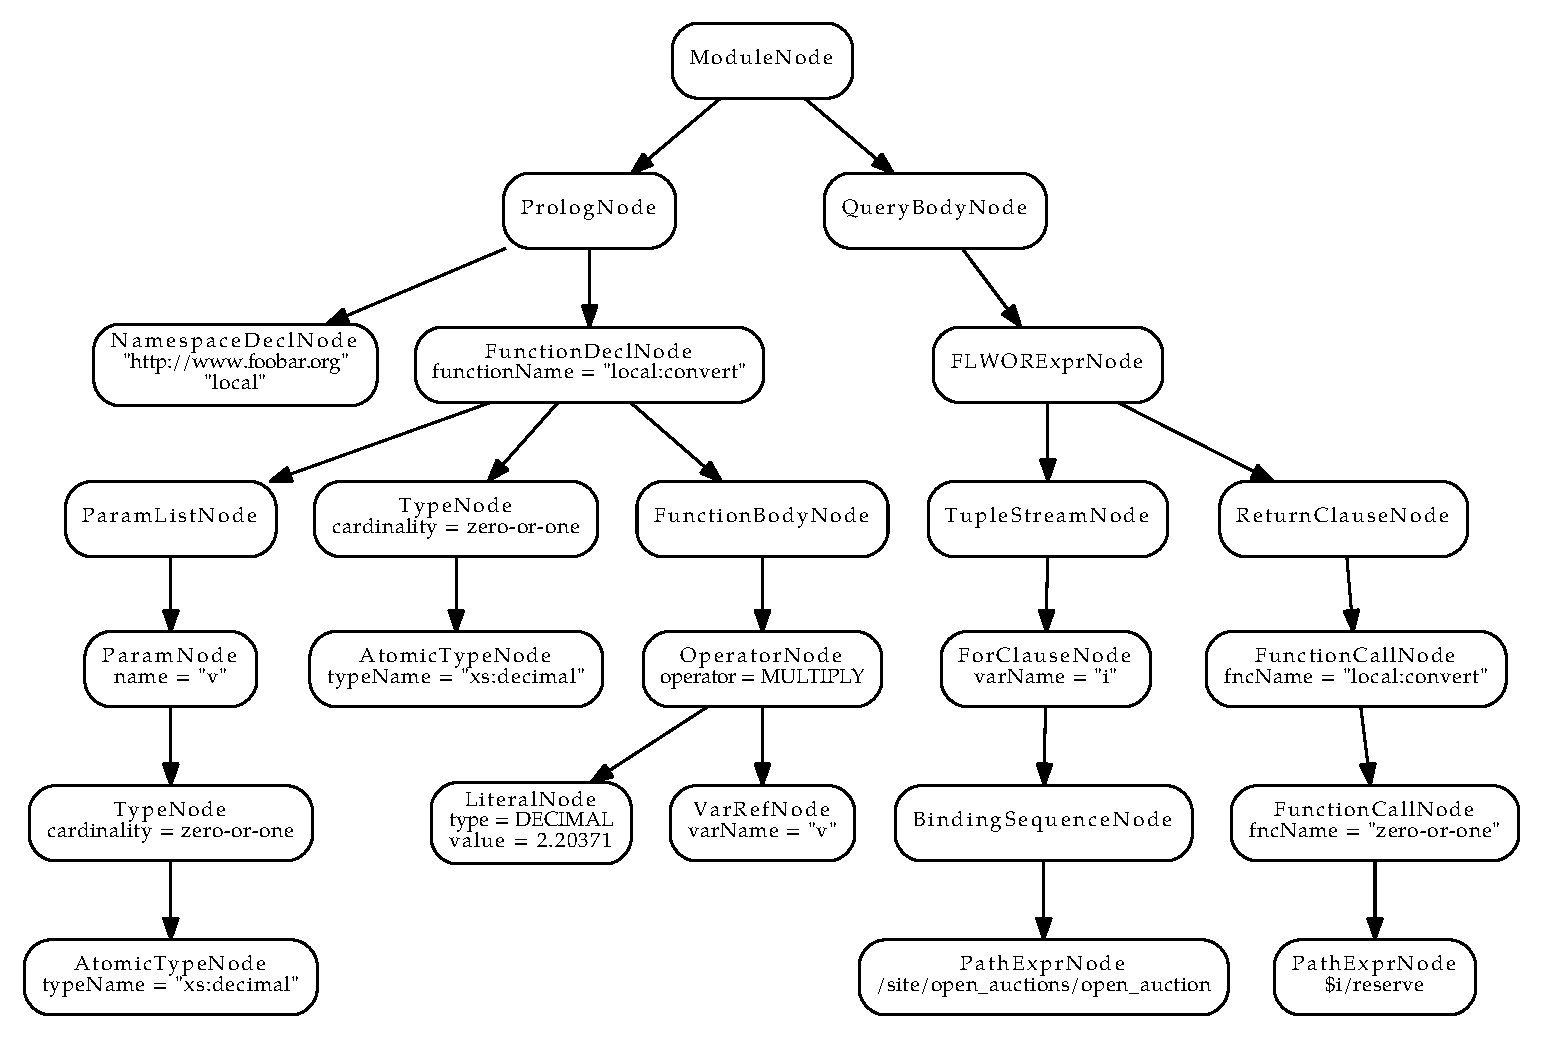
\includegraphics[scale=0.6]{syntax_tree_1.eps}
\end{figure}

A syntax tree constructed from sample query in Listing \ref{listing_sample_query_1} is shown in Figure \ref{FIG_syntax_tree_1}.

\section{Step 2: Static Analysis of Expression Types}
In the second step, we statically (i.e. without evaluation of the queries) determine types of expressions in the syntax tree. Information on the types of expressions can be used by consecutive steps of the algorithm. The consecutive steps will not use the determined types of all expressions, however this step may be useful in a future extending.

The analysis of expression types can be divided into three substeps. Determination of return types of functions, determination of types of global variables, and finally determination of types of expressions.

But firstly, we describe types of expressions we want to capture and their features.

\subsection{Expression Types}
\begin{itemize}
\item XML Schema built-in atomic types. See Attachment \ref{FIG_xsd_built_in_atomic_types}.
\item Types \emph{ElementType}, \emph{AttributeType}, \emph{NodeType}, \emph{TextNodeType},\linebreak \emph{CommentType}, \emph{ProcessingInstructionType}, \emph{DocumentType} representing an element, attribute, node, text node, comment, processing instruction, document node.
\item Type representing a node or a set of nodes selected by a certain path expression. The path expression is included in this type. Let this type be identified as \emph{PathType}.
\item \emph{UnknownType} representing a type without known details, which does not suit one of the three previous types. An example is XSD type \texttt{anyType}.
\end{itemize}

\subsection{PathType}
PathType contains additional information. The represented path is contained by an instance of \texttt{PathExprNode} containing list of its steps, in particular instances of \texttt{StepExprNode}. If a step is a reference to a variable which type is PathType, we also want to include this information. Therefore, PathType contain association between the steps and other PathTypes and this association is defined for the PathType variable steps.

To differ between a common PathType selecting a set of nodes and a PathType bound to a for variable in a FLWOR expression, PathType structure contains a flag \texttt{isForBound}.

Additionally, PathType contains a list of special functions that were called with an argument of PathType type. The motivation is that in some cases of function calls, we want to know that the function call is performed with an instance of PathType because then, we can determine a type of the function call more precisely. Those special functions are built-in functions \texttt{data}, \texttt{min}, \texttt{max}, \texttt{avg}, \texttt{sum}, \texttt{distinct-values}, \texttt{zero-or-one}, \texttt{exactly-one}. And other may be added, when needed.

In summary, we represent PathType as a structure with the following member variables.
\begin{itemize}
\item \texttt{pathExprNode} - An instance of \texttt{PathExprNode}.
\item \texttt{substeps} - An association between steps from \texttt{pathExprNode} and instances of PathType type.
\item \texttt{isForBound} - Boolean flag determining if the type was bound to a for variable in a for clause.
\item \texttt{specialFunctionCalls} - List of special functions called with this instance as an argument.
\end{itemize}

\subsection{Cardinality of Types}

To capture sequences, we assign the first two categories of types (all types except of PathType and UnknownType) with its cardinality as proposed in \cite{thesis_schejbal}. Each of those types can be perceived as a sequence. A type representing one value or one item can be perceived as a sequence of exactly one item. The cardinality expresses one of the following five sequence types.

\begin{itemize}
\item An empty sequence.
\item A sequence of exactly one item.
\item A sequence containing zero or one item (modifier \texttt{?}).
\item A sequence containing zero or more items (modifier \texttt{*}).
\item A sequence containing one or more items (modifier \texttt{+}).
\end{itemize}

PathType is not assigned with the cardinality since we do not evaluate the queries, and therefore, we cannot determine if a certain XQuery path targets zero, one or more nodes. Alike, UnknownType is neither assigned with the cardinality. Expressions of UnknownType are not utilized it the inference, therefore, their cardinality is not needed.

\subsection{Determination of Function Return Types}
Determination of return types of functions is needed because function calls can appear in expressions. A return type of a function can be determined at the moment the analysis of expressions encounters a call of the function; however, it involves multiple transitions of the syntax tree in a search for a definition of a particular function.

Instead, the syntax tree can be searched just once, before the analysis of expressions, and return types of all functions found are stored.

\begin{algorithm}
\caption{Function \texttt{getFunctionDeclarationNodes}: Retrieval of Function Declaration Nodes}
\label{ALG_retrieval_of_function_declaration_nodes}
\begin{algorithmic}[1]
\REQUIRE $syntaxTree$: A reference to the root node of a syntax tree.
\ENSURE A list of syntax tree nodes representing function declarations.

\STATE $prologNode :=$ null
\FORALL{$moduleChildNode \in syntaxTree.getChildren()$}
    \IF{$is(moduleChildNode,$ PrologNode$)$}
        \STATE $prologNode := moduleChildNode$
    \ENDIF
\ENDFOR

\STATE $functionDeclarationNodes :=$ an empty list
\IF{$prologNode \neq$ null}
    \FORALL{$prologChildNode \in prologNode.getChildren()$}
        \IF{$is(prologChildNode,$ FunctionDeclNode$)$}
            \STATE add $prologChildNode$ to $functionDeclarationNodes$
        \ENDIF
    \ENDFOR
\ENDIF

\RETURN functionDeclarationNodes
\end{algorithmic}
\end{algorithm}

A simple algorithm is presented in Algorithm \ref{ALG_processing_of_functions}. It uses\linebreak \texttt{getFunctionDeclarationNodes} function, defined in Algorithm \ref{ALG_retrieval_of_function_declaration_nodes}, which returns a list of all function declaration nodes in the syntax three. Actually, it does not have to search the whole syntax tree as the function declaration nodes can be present only in the query prolog section. 

Without loss of generality, we will focus on locally defined functions. We will not determine types of functions defined in other modules since the principle is similar but it is needed to look up the definitions in syntax trees of other queries. Return types of built-in functions are fixed and, thus, there is no need to analyse them. Also, since a determination of a prefix for built-in functions is a technical issue, we assume that built-in functions are either prefixed by \texttt{fn} or not prefixed.

\begin{algorithm}
\caption{Processing of Functions}
\label{ALG_processing_of_functions}
\begin{algorithmic}[1]
\REQUIRE $syntaxTree$: A reference to the root node of a syntax tree.
\ENSURE An associative array of function names with their types and references to the their declaration nodes.

\STATE $functionArray :=$ an empty associative array
\FORALL{$functionDeclarationNode \in$ \\ $getFunctionDeclarationNodes(syntaxTree)$}
    \STATE $functionName := functionDeclarationNode.funcName$
    \STATE $typeNode := functionDeclarationNode.getChild(TypeNode)$
    \STATE $functionArray[functionName] :=$ \\ $(getTypeTN(typeNode), functionDeclarationNode)$
\ENDFOR
\RETURN $functionArray$
\end{algorithmic}
\end{algorithm}

\begin{algorithm}
\caption{Function \texttt{getTypeTN}: Extraction of a Type from TypeNode}
\label{ALG_extraction_of_a_type_from_typenode}
\begin{algorithmic}[1]
\REQUIRE $typeNode$: Syntax tree node of TypeNode class.
\ENSURE Type extracted from $typeNode$.

\STATE $type :=$ UnknownType
\STATE $cardinality := typeNode.cardinality$
\STATE $itemTypeNode := typeNode.getChild(ItemTypeNode)$
\IF{$is(itemTypeNode,$ AtomicTypeNode$)$}
    \STATE $type :=$ XSD atomic built-in type $itemTypeNode.typeName$, $cardinality$
\ELSIF{$is(itemTypeNode,$ KindTestNode$)$}
    \STATE $type := itemTypeNode.nodeKind$, $cardinality$
\ENDIF

\RETURN $type$
\end{algorithmic}
\end{algorithm}

For the rest of the thesis, we assume function \texttt{getFunctionReturnType} which takes a function name and returns the return type of the function if the function is either built-in or it is recorded in the associative array. Otherwise, \texttt{null} is returned.

Later phases of the algorithm need to process the declarations of certain functions. Therefore, we also store references to the entire function declaration nodes, accessible using function \texttt{getFunctionDeclNode}.

\subsection{Auxiliary Functions}
Before proceeding to the next phase of the algorithm, we introduce auxiliary functions used in pseudo algorithms.

Function \texttt{memorizeType} takes two arguments \texttt{node} and \texttt{type} and it memorizes the given type of the specified expression node. This information can be then retrieved by function \texttt{getType}, specifying the particular node as its argument.

Another group consists of functions \texttt{set}, \texttt{add}, and \texttt{get}. Function \texttt{set} memorizes a given value of a specified property of a specified node. It is used to assign a node with a named value, for example, \texttt{set(someNode, color, "red")} will assign \texttt{someNode} with string value \texttt{"red"} which can be then retrieved by function \texttt{get}, specifying the node and the property name. For example,\linebreak \texttt{get(someNode, color)} returns \texttt{"red"}. A subsequent call of \texttt{set} assigning a node with a value of already assigned property will overwrite it, leaving the property with the newer value. However, a property can have several values and this can be achieved using function \texttt{add} with the same syntax as function \texttt{set} but instead of overwriting the existing property, \texttt{add} will append the new value to the existing ones. Then, a call of \texttt{get} on this node and property returns a list of all its values, preserving the order of their addition.

\subsection{Determination of Global Variable Types}
A similar approach as in the case of functions can be applied to determine types of global variables. Alike the functions, the global variables are defined in the prolog section. A type of a variable can be explicitly specified in its definition, for instance \texttt{declare variable \$x as xs:byte := 12;}. If it is not, it may often be deducible from the binding expression. Again, we do not analyse external variables for the same reason as in case of external functions.

\begin{algorithm}
\caption{Function \texttt{determineExpressionType}}
\label{ALG_func_determineExpressionType}
\begin{algorithmic}[1]
\REQUIRE{\ \\
    $exprNode$: An expression node in the syntax tree. \\
    $contextVarTypes$: Types of local variables valid in the current subtree.
}
\ENSURE The expression type.

\STATE $type :=$ UnknownType
\IF{$is(exprNode,$ LiteralNode$)$}
     \STATE $type :=$ XSD atomic type $exprNode.type$, exactly-once cardinality
\ELSIF{$is(exprNode,$ FunctionCallNode$)$}
     \STATE $type := getFunctionReturnType(exprNode.fncName)$
\ELSIF{$is(exprNode,$ VarRefNode$)$}
     \STATE $type := getVariableType(contextVarTypes, exprNode.varName)$
     \IF{$type$ is PathType}
         \STATE $step :=$ a path step (new instance of StepExprNode) representing the variable reference
		 \STATE $substeps :=$ an empty associative array         
         \STATE $substeps[step] := type$
         \STATE $pathExprNode :=$ new instance of PathExprNode containing one step step
         \STATE $type :=$ PathType containing $pathExprNode$ and $substeps$
     \ENDIF
\ELSIF{$is(exprNode,$ PathExprNode$)$}
     \STATE $type := createPathType(exprNode)$
\ELSIF{$is(exprNode,$ OperatorNode$)$}
     \STATE $type := determineOperatorType(exprNode, contextVarTypes)$
\ELSIF{$is(exprNode,$ FLWORExprNode$)$}
     \STATE $returnClauseNode := exprNode.getChild(ReturnClauseNode)$
     \STATE $type := createForUnboundType(getType(returnClauseNode))$
\ENDIF

\RETURN type
\end{algorithmic}
\end{algorithm}

\begin{algorithm}
\caption{Function \texttt{determineOperatorType}}
\label{ALG_func_determineOperatorType}
\begin{algorithmic}[1]
\REQUIRE{\ \\ 
    $operatorNode$: An operator expression node in the syntax tree. \\
    $contextVarTypes$: Types of local variables valid in the current subtree.
}
\ENSURE The operator expression type.

\STATE $type :=$ UnknownType
\STATE $operator := operatorNode.operator$
\IF{$isOperatorClassComparison(operator)$}
    \STATE $type :=$ boolean, exactly-one cardinality
\ELSIF{$isOperatorClassAddition(operator)$}
    \STATE $leftOperandType := getType(exprNode.leftSide)$
    \STATE $rightOperandType := getType(exprNode.rightSide)$
    \IF{$isNumericType(leftOperandType)$ \\ $\wedge$ $isNumericType(rightOperandType)$}
        \STATE $type := selectMoreGeneralNumericType(leftOperandType,$ $rightOperandType)$
    \ELSIF{$isNumericType(leftOperandType)$}
        \STATE $type := leftOperandType$
    \ELSIF{$isNumericType(rightOperandType)$}
        \STATE $type := rightOperandType$
    \ENDIF
\ENDIF

\RETURN type
\end{algorithmic}
\end{algorithm}

\begin{algorithm}
\caption{Function \texttt{isOperatorClassComparison}}
\label{ALG_func_isOperatorClassComparison}
\begin{algorithmic}[1]
\REQUIRE $operator$: A representation of a XQuery operator.
\ENSURE true if $operator$ is a comparison operator, false otherwise.

\IF{$operator$ equals one of GEN\_EQUALS, GEN\_GREATER\_THAN, GEN\_GREATER\_THAN\_EQUALS, GEN\_LESS\_THAN, GEN\_LESS\_THAN\_EQUALS, GEN\_NOT\_EQUALS, VAL\_EQUALS, VAL\_GREATER\_THAN, VAL\_GREATER\_THAN\_EQUALS, VAL\_LESS\_THAN, VAL\_LESS\_THAN\_EQUALS, VAL\_NOT\_EQUALS}
    \RETURN true
\ELSE
    \RETURN false
\ENDIF
\end{algorithmic}
\end{algorithm}

\begin{algorithm}
\caption{Function \texttt{isOperatorClassAddition}}
\label{ALG_func_isOperatorClassAddition}
\begin{algorithmic}[1]
\REQUIRE $operator$: A representation of a XQuery operator.
\ENSURE true if $operator$ is an addition operator, false otherwise.

\IF{$operator$ equals one of PLUS, MINUS, UNARY\_PLUS, UNARY\_MINUS}
    \RETURN true
\ELSE
    \RETURN false
\ENDIF
\end{algorithmic}
\end{algorithm}

\begin{algorithm}
\caption{Function \texttt{isNumericType}}
\label{ALG_func_isNumericType}
\begin{algorithmic}[1]
\REQUIRE $type$: A representation of a type.
\ENSURE true if $type$ represents one of the XSD atomic built-in numeric types, false otherwise.

\IF{$type$ represents one of float, double, decimal, integer, long, int, short, byte, nonPositiveInteger, negativeInteger, nonNegativeInteger, positiveInteger, unsignedLong, unsignedInt, unsignedShort, unsignedByte}
    \RETURN true
\ELSE
    \RETURN false
\ENDIF
\end{algorithmic}
\end{algorithm}

The algorithm iterates through the variable declaration nodes from the prolog and if the variable is explicitly assigned with its type, the type is noted. Otherwise, an attempt of the type deduction of the binding expression is made. The deduction of the type from the expression is presented in Algorithm \ref{ALG_func_determineExpressionType}. On input, it takes an expression node and types of local variables that are valid in the expression (also called context of variables or variable context). The presented algorithm is just shortened illustration since the complete version is too long to be presented in this text. Nevertheless, the principle is straightforward. Depending on the class of the expression node (show in Figure \ref{FIG_syntax_tree_node_types_part_1}), its type can be either determined directly or it depends on its subexpressions.

The meaning of the code at lines 6-14 is the following. If a variable is bound to an expression which type is PathType, we want to assign the variable reference expression with PathType which represents path containing exactly one step, the variable reference. Some algorithm in later sections search for paths starting with a certain variable and we want them to include also that types of expressions.	

A part of the function's semantic is separated in Algorithm \ref{ALG_func_determineOperatorType}, which is not presented completely because of the same reason.

Function \texttt{determineExpressionType} is called within function \texttt{analysis\-Of\-Expression\-Types} presented in Algorithm \ref{ALG_func_analysisOfExpressionTypes}, which recursively determines types of all subexpressions. Two important questions about this function emerge. How (in which order) are the tree nodes recursively processed and how does the function handle definitions (bindings) of new variables which may also appear in the expressions?

The order of the recursion is firstly to process children of a node and then the node itself. The order of child processing is specified by function $o$ from the definition of the syntax tree in Definition \ref{DEF_syntax_tree}. The reason is that an expression node may need to know types of its subexpressions to determine its own type and we want to determine types of all expressions. Therefore, using the described order, subexpressions of an expression are processed first, and then the expression itself without any need for further recursion, because the types of the subexpressions are already determined.

The handling of new variable definitions relies on the fact that the definitions make the new variables valid only in nodes with a higher sequence number when numbered in the order described in in the previous paragraph. Therefore, the left-most (the first amongst the ordered subnodes) subnode of a certain node can be processed without an extension of the variable context. And, if the left-most subnode extends the variable context for the following nodes in the numbering, it can be easily handled because the types of the new variables can be directly determined since the binding expressions are already processed (thus, their types are known). Every node ''knows'' whether or not it may define new variables for nodes with higher sequence numbers. This is expressed in the algorithm by the condition stating at line 10. If it does define new variables, they are memorized. Later, upon processing of its parent, they are retrieved and the variable context is extended. This is done at lines 4 and 5. Function \texttt{mergeContextVarTypes} presented in Algorithm \ref{ALG_function_mergeContextVarTypes} writes every record from its second argument (the new variables) into its first argument (the variable context). If there are records for variables with the same names in the context, they are overwritten to correspond to the variable overlapping. It is important to note that we assume the variable context is not passed by reference but by value, and hence, the variable context of a certain node is not affected by the recursive processing of its subnodes.

\begin{algorithm}
\caption{Function \texttt{analysisOfExpressionTypes}}
\label{ALG_func_analysisOfExpressionTypes}
\begin{algorithmic}[1]
\REQUIRE{\ \\
    $startingNode$: A node determining a subtree to perform the analysis on. \\
    $contextVarTypes$: Types of local variables valid in the current subtree.
}

\FORALL{$i \in \{1, \dots, |startingNode.getChildren()|\}$ ordered from the lowest to the highest}
    \STATE $subnode := startingNode.getChild(i)$
    \STATE $analysisOfExpressionTypes(subnode, contextVarTypes)$ \COMMENT{recursion}
    \STATE $newVars := get(subnode, newVars)$    
    \STATE $contextVarTypes := mergeContextVarTypes(contextVarTypes, newVars)$
\ENDFOR
\IF{$is(startingNode,$ ExprNode$)$}
    \STATE $memorizeType(startingNode, determineExpressionType(startingNode))$
\ENDIF
\IF{$is(startingNode,$ VariableBindingNode$)$}
    \STATE $type :=$ null
    \STATE $typeNode := startingNode.getChild(TypeNode)$
    \IF{$typeNode \neq null$}
        \STATE $type := getTypeTN(typeNode)$
    \ELSE
        \STATE $type := determineExpressionType(startingNode.$ $getChild(BindingSequenceNode).getChild(ExprNode),$ $contextVarTypes)$
        \IF{$is(startingNode,$ ForClauseNode$)$}
            \STATE $type := createForBoundType(type)$
        \ENDIF
    \ENDIF
    \STATE $set(startingNode, newVars, (startingNode.varName, type))$
\ELSIF{$is(startingNode,$ TupleStreamNode$) \vee is(startingNode,$ InClausesNode$)$}
    \FORALL{$varBindingNode \in startingNode.getChildren()$}
        \STATE $add(startingNode, newVars, get(varBindingNode, newVars))$
    \ENDFOR
\ENDIF
\end{algorithmic}
\end{algorithm}

\begin{algorithm}
\caption{Function \texttt{mergeContextVarTypes}}
\label{ALG_function_mergeContextVarTypes}
\begin{algorithmic}[1]
\REQUIRE{\ \\
    $contextVarTypes$: Types of local variables valid in current context. \\    
    $extendingVarTypes$: New variables in the same structure as the first argument.
}
\ENSURE The context variable types extended with the variable types from the second argument.

\FORALL{$varName \in keys(extendingVarTypes)$}
    \STATE $contextVarTypes[varName] := extendingVarTypes[varName]$
\ENDFOR
\RETURN $contextVarTypes$
\end{algorithmic}
\end{algorithm}

Function \texttt{analysisOfExpressionTypes} called upon a binding expression of a global variable determines the type of the binding expression, and hence, the type of the variable. In case of global variables, the argument \texttt{contextVarTypes} is empty, because there are no local variables valid in the prolog section.

\begin{algorithm}
\caption{Function \texttt{getVariableType}}
\label{ALG_function_get_variable_type}
\begin{algorithmic}[1]
\REQUIRE{\ \\
    $contextVarTypes$: Types of local variables valid in current context. \\
    $var$: A variable to determine the type of.
}
\ENSURE The type of variable $var$.

\IF{$contextVarTypes[var]$ is defined}
     \RETURN $contextVarTypes[var]$
\ELSE
     \RETURN $getGlobalVariableType(var)$
\ENDIF
\end{algorithmic}
\end{algorithm}

The types of processed global variables are available trough function \linebreak \texttt{getGlobalVariableType}. If the function gets a variable that is not a global one, it returns \texttt{null}. Function \texttt{getVariableType} called in Algorithm \ref{ALG_func_determineExpressionType} is defined in Algorithm \ref{ALG_function_get_variable_type}. It checks if the specified variable is amongst the given local variables. If so, it returns its type, else it handles the variable as a global one and if such global variable does not exist the result is \texttt{null}.

\begin{algorithm}
\caption{Function \texttt{createPathType}}
\label{ALG_function_create_path_type}
\begin{algorithmic}[1]
\REQUIRE $pathExprNode$: A reference to a PathExprNode to create the PathType from.
\ENSURE The PathType of $pathExprNode$ expression.

\STATE $stepNodes :=$ an empty array
\STATE $forBoundSubsteps :=$ an empty associative array
\FORALL{$stepNode \in pathExprNode.getChildren()$}
	\STATE $detailNode := stepNode.getChild(ExprNode)$
	\IF{$detailNode \neq$ null}
		\IF{$is(detailNode,$ VarRefNode$)$}
			\STATE $type := getType(detailNode)$ \COMMENT{PathType}
			\IF{$type.isForBound$}
				\STATE $forBoundSubsteps[stepNode] := type$
				\STATE add $stepNode$ to $stepNodes$
			\ELSE
				\STATE add all $type.stepNodes$ to $stepNodes$
			\ENDIF
		\ELSE
			\STATE add $stepNode$ to $stepNodes$
		\ENDIF
	\ELSE
		\STATE add $stepNode$ to $stepNodes$
	\ENDIF
\ENDFOR

\RETURN $PathType$ with $stepNodes$, $forBoundSubsteps$, and $isForBound$ set to false
\end{algorithmic}
\end{algorithm}

\subsection{Determination of Expression Types}
To determine types of expressions, we use already introduced function \\ \texttt{analysisOfExpressionTypes}. The starting node (its first argument) is the node representing the query body and the variable context is empty as there cannot be any local variable valid in the body node.

\begin{algorithm}
\caption{Function \texttt{createForBoundType}}
\label{ALG_function_create_for_bound_type}
\begin{algorithmic}[1]
\REQUIRE $type$: A type to create the for bound type from.
\ENSURE The for bound type from $type$.

\IF{$type$ is UnknownType}
	\RETURN UnknownType
\ELSIF{$type$ is NodeType or XSD atomic type}
	\RETURN $type$ with cardinality set to exactly-one
\ELSE
	\STATE \COMMENT {It is PathType}
	\RETURN $type$ with $isForBound$ flag set to true
\ENDIF
\end{algorithmic}
\end{algorithm}

\begin{figure}
\label{FIG_syntax_tree_1_types}
\caption{Sample syntax tree 1 after the static analysis of types.}
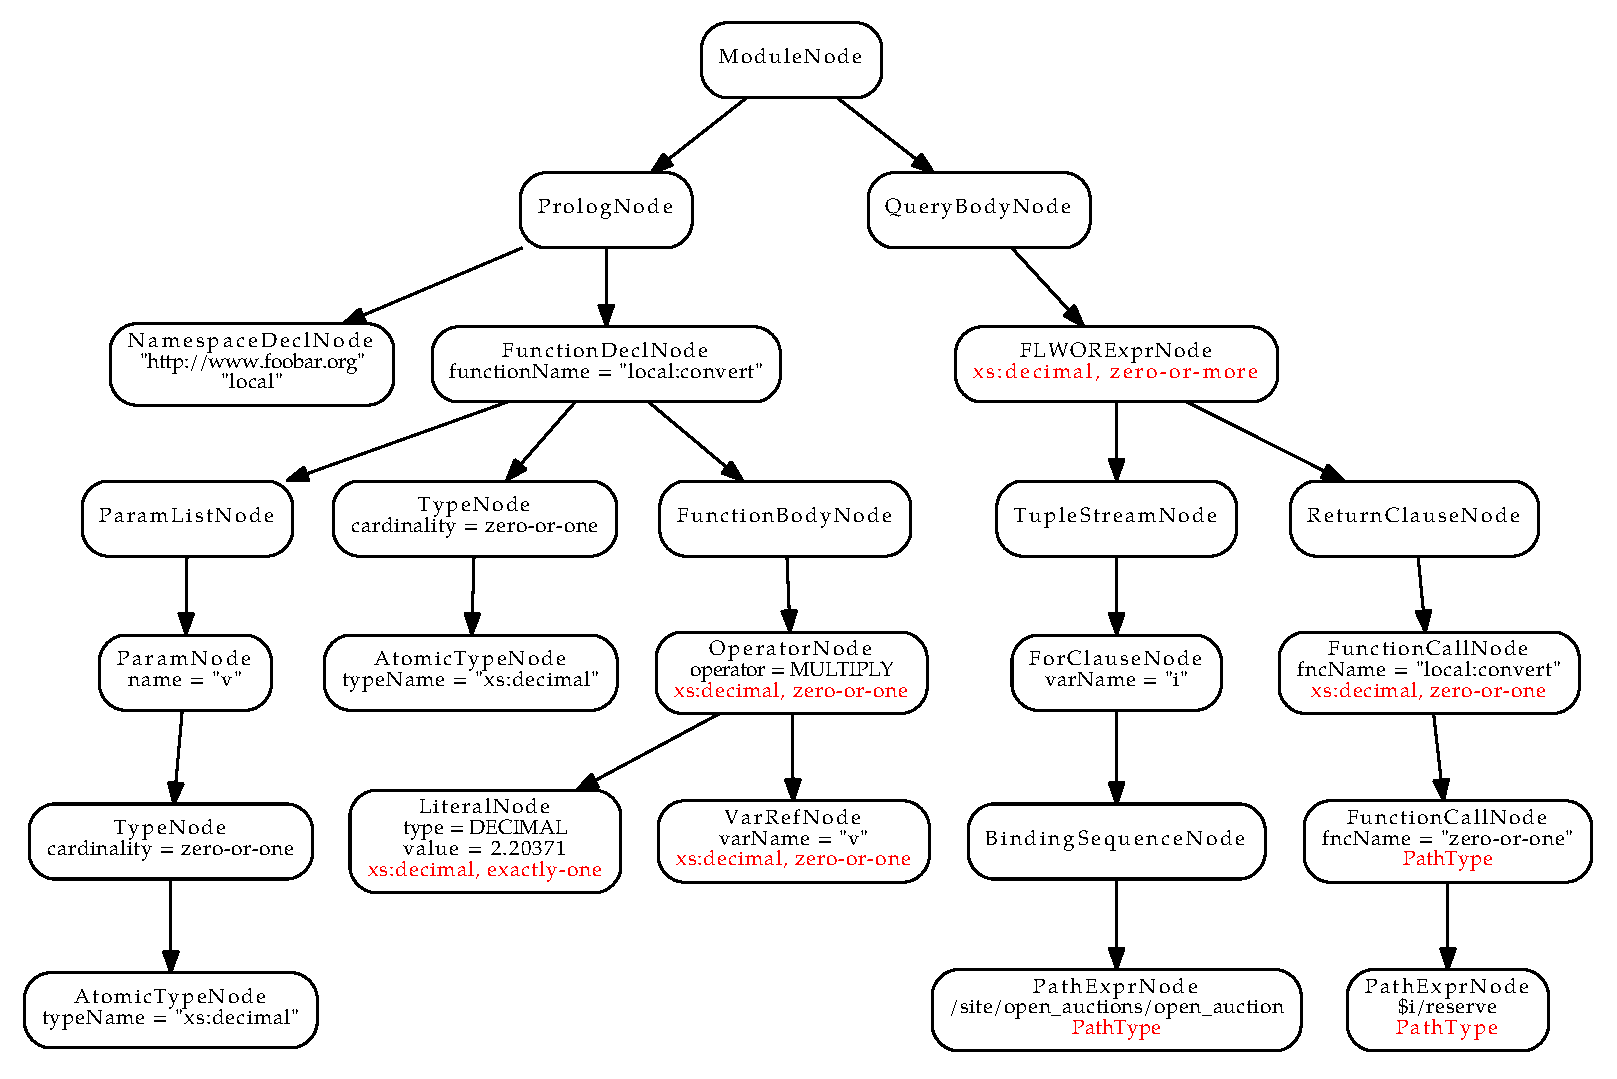
\includegraphics[scale=0.5]{syntax_tree_1_types.eps}
\end{figure}

We can also determine expression types in functions. To do this for a certain function, \texttt{analysisOfExpressionTypes} function has to be called with a function declaration node as the starting node. In this case, the function declaration node contains a subnode specifying function's formal arguments. These argument are set as the variable context for the function body represented by another subnode.

Figure \ref{FIG_syntax_tree_1_types} shows the syntax tree from Figure \ref{FIG_syntax_tree_1} after the static analysis of expression types. The types are shown in red color. Note that the node representing \texttt{zero-or-one} function call is of a PathType type, as well as its argument. It is so, because the function returns its argument unchanged, and thus, we included the function in the special functions list in the PathType definition.

Also note, that the function call node of \texttt{local:convert} in the FLWOR return clause has \texttt{zero-or-one} cardinality and the FLWOR node has \texttt{zero-or-more} cardinality. The change of cardinality is a result of the for unbinding shown in Algorithm \ref{ALG_function_create_for_unbound_type}.

\begin{algorithm}
\caption{Function \texttt{createForUnboundType}}
\label{ALG_function_create_for_unbound_type}
\begin{algorithmic}[1]
\REQUIRE $type$: A type to create the for unbound type from.
\ENSURE The for unbound type from $type$.

\IF{$type$ is UnknownType}
	\RETURN UnknownType
\ELSIF{$type$ is NodeType or XSD atomic type}
	\RETURN $type$ with cardinality set to zero-or-more
\ELSE
	\STATE \COMMENT {It is PathType}
	\RETURN $type$ with $isForBound$ flag set to false
\ENDIF
\end{algorithmic}
\end{algorithm}

\section{Step 3: Inference of Built-in Types}
In this step, the algorithm goes through the syntax tree to infer types of elements and attributes from expressions using the type information from the previous step. These two steps could be merged together but for better comprehension we present it separately.

How are the types inferred from the expression types? We do not exploit all expressions. Only expressions of a particular type are exploited. Specifically, an expression has to contain an subexpression $E$ of PathType type (expression representing a certain element or attribute or set of elements or attributes). In the following text, the set represented by expression $E$ is denoted $S$. Another requirement is that the expression has to be either a function call or an arithmetic operation. As discussed in Chapter \ref{CHAPTER_analysis_of_xquery}, also other XQuery constructs can be utilized to infer built-in types, but, since the principle is similar, we focus on the two mentioned.

The output of this step is a set of statements of form $P \rightarrow T$, where $P$ is an instance of PathType and $T$ is an XML Schema built-in atomic type.

\subsection{Function Calls}\label{SUBSECTION_function_calls}
This case is quite straightforward. The algorithm encounters a function call and one of the arguments is a set of elements of attributes (subexpression $E$ representing $S$) represented by PathType $p$. To determine the type of $S$, it is only needed to determine the type of the corresponding formal argument from the definition of the function. The function is either a built-in one so its definition is known or it is defined in the prolog section. External functions are not processed as was mentioned already.

If the type $t$ of the formal argument is a built-in type or its sequence, then $t$ is also the inferred type of $S$. The inferred statement is $p \rightarrow t$. Otherwise, no statement is inferred.

\subsection{Arithmetic Operations}
If the operator in an arithmetic operation is one of \texttt{+}, \texttt{-}, \texttt{div}, \texttt{mod}, \texttt{*}, \texttt{/} (the class of the expression node is \texttt{Operator} and it represents one of \texttt{PLUS}, \texttt{MINUS}, \texttt{IDIV}, \texttt{MOD}, \texttt{MUL}, \texttt{DIV} (for all operators, see Attachment \ref{FIG_operators})), one operand is of PathType $p$ and the type $t$ of the other operand is one of numeric built-in types, then the inferred statement is $p \rightarrow t$.

If the operator is one of \texttt{<}, \texttt{>}, \texttt{<=}, \texttt{>=}, \texttt{=}, \texttt{!=} (the class of the expression node is \texttt{Operator} and it represents one of \texttt{GEN\_LESS\_THAN}, \texttt{GEN\_GREATER\_THAN}, \texttt{GEN\_LESS\_THAN\_EQUALS}, \texttt{GEN\_GREATER\_THAN\_EQUALS}, \texttt{GEN\_EQUALS}, \\ \texttt{GEN\_NOT\_EQUALS}), one operand is of PathType $p$ and the type $t$ of the other operand is one of built-in types, then the inferred statement is $p \rightarrow t$.

\subsection{Example}

\begin{figure}
\label{FIG_syntax_tree_1_types_type_inference}
\caption{Example of an inference of a type from a function call.}
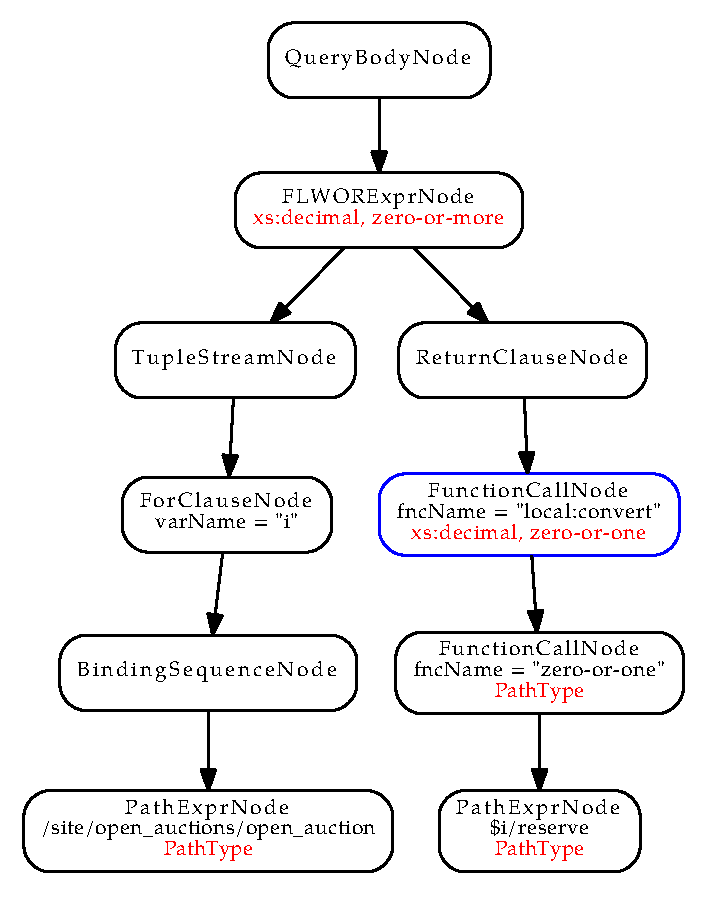
\includegraphics[scale=1]{syntax_tree_1_types_type_inference.eps}
\end{figure}

Figure \ref{FIG_syntax_tree_1_types_type_inference} shows a fraction of the syntax tree from Figure \ref{FIG_syntax_tree_1_types}. When the inference of built-in types encounters the node marked by blue color, a statement will be inferred using the principle described in Chapter \ref{SUBSECTION_function_calls}. The node represents a call of \texttt{local:convert} function.

This function has one formal argument of type $t =$ \texttt{xs:decimal}, \texttt{zero-or-one} cardinality. The real argument is of a PathType $p$. In particular, it is a PathType representing path \texttt{\$i/reserve}, where the \texttt{\$i} variable refers to a PathType representing for-bound \texttt{/site/open\_auctions/open\_auction} path, and one special function call of \texttt{zero-or-one} function is noted.

Since the criteria for the inference from a function call are met, statement $p \rightarrow t$ is inferred.

\subsection{Possible Extensions}
As mentioned, the proposed algorithm utilizes only a small portion of XQuery constructs which can be be possibly utilized. Also, the algorithm does not perform the inference of types inside user-defined functions (it just uses the return types determined in earlier phases). That can be easily done as we know the definitions of functions and types of their real arguments. An algorithm performing the analysis in the user-defined functions can works as follows.

If a currently processed expression is a function call of an user-defined function and at least one of its real arguments is an instance of PathType, get the function declaration node. In the function body, replace the formal arguments by the real arguments and set them as the local variables, so the proposed algorithms can be applied to process the function's body. Analyse the types of expressions in the body with the new information on the types of arguments by incorporating of the proposed algorithms and replace the function's return type by the one currently determined.

A little complication is a recursion. A simple algorithm of that kind may never end because of the infinite analysis of the same recursive function(s). Therefore, we shall keep track of the currently analysed functions (e.g. in a stack of function calls) and do not process the recursive calls. 

\section{Step 4: Key Discovery}
In this step, the algorithm discovers keys of elements, incorporating the approach from paper \cite{Necasky:2009:DXK:1529282.1529414}, described in Chapter \ref{Keys}, and extending it. Firstly, the syntax tree is searched for forms of FLWOR expressions to infer the keys from. Then, as described later, certain constructs are used to support or degrade the evidence of inferred statements in a final summary.

\subsection{Auxiliary Functions} \label{step_4_auxiliary_functions}
Firstly, we define some auxiliary functions used by algorithms in this chapter.

Function \texttt{usesOnlyChildAndDescendantAxes} in Algorithm \ref{ALG_function_uses_only_child_and_descendant_axes} takes an instance of PathType as its arguments and returns true if the path uses only child and descendant axes. Otherwise, it returns false.

\begin{algorithm}
\caption{Function \texttt{usesOnlyChildAndDescendantAxes}}
\label{ALG_function_uses_only_child_and_descendant_axes}
\begin{algorithmic}[1]
\REQUIRE $pathType$: A PathType instance.
\ENSURE A boolean result.

\FORALL{$stepNode \in pathType.stepNodes$}
	\IF{$stepNode.isAxisStep$}
		\STATE $axisKind := stepNode.axisNode.getAxisKind()$
		\IF{$axisKind \neq$ CHILD $\wedge$ $axisKind \neq$ DESCENDANT}
			\RETURN false
		\ENDIF
	\ENDIF
\ENDFOR

\STATE $detailNode := stepNode.getChild(ExprNode)$
\IF{$detailNode \neq$ null}
	\IF{$is(detailNode,$ VarRefNode$)$}
		\IF{$usesOnlyChildAndDescendantAxes($ $pathType.forBoundSubsteps[stepNode]) =$ false}
			\RETURN false
		\ENDIF
	\ENDIF
\ENDIF

\RETURN true
\end{algorithmic}
\end{algorithm}

Function \texttt{isWithoutPredicates} in Algorithm \ref{ALG_function_is_without_predicates} checks whether a path represented by a given PathType instance does not contain predicates. A Similar function is  \texttt{isWithoutPredicatesExceptLastStep}. This function is not explicitly defined, because its definition is the same as the definition of function \texttt{isWithoutPredicates}, except it does not check the last step of the path. So the last step may contain predicates and the function will return true.

\begin{algorithm}
\caption{Function \texttt{isWithoutPredicates}}
\label{ALG_function_is_without_predicates}
\begin{algorithmic}[1]
\REQUIRE $pathType$: A PathType instance.
\ENSURE A boolean result.

\FORALL{$stepNode \in pathType.stepNodes$}
	\IF{$stepNode.hasPredicates$}
		\RETURN false
	\ENDIF
	\IF{$pathType.forBoundSubsteps[stepNode] \neq$ null}
		\IF{$isWithoutPredicates(pathType.forBoundSubsteps[stepNode] =$ false}
			\RETURN false
		\ENDIF
	\ENDIF
\ENDFOR

\RETURN true
\end{algorithmic}
\end{algorithm}

Function \texttt{endsWithExactlyOnePredicate} in Algorithm \ref{ALG_function_ends_with_exactly_one_predicate} checks if a path represented by a given PathType instance contains exactly one predicate in its last step and if so, the predicate is returned. Otherwise, it returns false.

\begin{algorithm}
\caption{Function \texttt{endsWithExactlyOnePredicate}}
\label{ALG_function_ends_with_exactly_one_predicate}
\begin{algorithmic}[1]
\REQUIRE $pathType$: A PathType instance.
\ENSURE If $pathType$ ends with exactly one predicate, return value is the predicate, otherwise return value is false.

\STATE $lastStepNode :=$ the last item from $pathType.stepNodes$
\IF{$lastStepNode.hasPredicates() =$ false}
	\RETURN false
\ENDIF
\IF{number of items in list $lastStepNode.getChild(PredicateListNode)$ $.getChildren()$ is higher than 1}
	\RETURN false
\ENDIF

\RETURN the only item in $lastStepNode.getChild(PredicateListNode)$ $.getChildren()$
\end{algorithmic}
\end{algorithm}

Function \texttt{isTargetPath} in Algorithm \ref{ALG_function_is_target_path} checks if a path represented by a given PathType instance is so-called target path for the specified variable. A target path for a variable is a path where its first step is a reference to the variable.

\begin{algorithm}
\caption{Function \texttt{isTargetPath}}
\label{ALG_function_is_target_path}
\begin{algorithmic}[1]
\REQUIRE{\ \\
  $pathType$: A PathType instance. \\
  $varName$: A variable name.
}
\ENSURE Returns true, if the first step of path represented by the PathType instance is a reference to the specified variable.

\STATE $firstStep :=$ first item from  $pathType.stepNodes$
\STATE $detailNode := firstStep.detailNode$
\IF{$detailNode =$ null}
	\RETURN false
\ENDIF
\IF{$is(detailNode,$ VarRefNode$) =$ false}
	\RETURN false
\ENDIF
\IF{$detailNode.varName = varName$}
	\RETURN true
\ELSE
	\RETURN false
\ENDIF
\end{algorithmic}
\end{algorithm}

Function \texttt{getTargetReturnPathTypes} in Algorithm \ref{ALG_function_get_target_return_path_types} searches the given FLWOR for PathTypes representing so-called target return paths. A target return path is a return path in a where clause of a FLWOR. The FLWOR is processed recursively using function \texttt{getTargetReturnPathTypesRecursive} in Algorithm \ref{ALG_function_get_target_return_path_types_recursive}.

\begin{algorithm}
\caption{Function \texttt{getTargetReturnPathTypes}}
\label{ALG_function_get_target_return_path_types}
\begin{algorithmic}[1]
\REQUIRE{\ \\
  $flworNode$: A FLWORExprNode instance to search for target return paths. \\
  $varName$: A variable name.
}
\ENSURE A list of target return paths for the specified variable, in the given FLWOR, represented by PathType instances.

\STATE $pathTypes :=$ an empty array
\STATE $getTargetReturnPathTypesRecursive(flworNode.$ $getChild(ReturnClauseNode), varName, pathTypes)$
\RETURN $pathTypes$
\end{algorithmic}
\end{algorithm}

\begin{algorithm}
\caption{Function \texttt{getTargetReturnPathTypesRecursive}}
\label{ALG_function_get_target_return_path_types_recursive}
\begin{algorithmic}[1]
\REQUIRE{\ \\
  $node$: A node to search for target return paths. \\
  $varName$: A variable name. \\
  $pathTypes$ An output list to add found target return path types to.
}

\IF{$is(node,$ ExprNode$)$}
	\STATE $type := getType(node)$
	\IF{$type$ is $PathType$ $\wedge$ $isTargetPath(type, varName)$}
		\STATE add $type$ to $pathTypes$
	\ENDIF
\ENDIF
\FORALL{$child \in node.getChildren()$}
	\STATE $getTargetReturnPathTypesRecursive(child, varName, pathTypes)$
\ENDFOR
\end{algorithmic}
\end{algorithm}

A similar couple of functions is function \texttt{getTargetReturnPaths} and function \texttt{getTargetReturnPathsRecursive}. Only difference between those two couples of functions is that the former one searches for all expressions which are of PathType representing a target return path, while the later one searches only for instances of \texttt{PathExprNode}.

To illustrate this difference, we introduce the following example. Assuming $P$ is a return target path expression for variable $var$ and $flwor$ is a FLWOR expression with return clause \texttt{data(}$P$\texttt{)}, function call \texttt{getTargetReturnPathTypes(} $flwor$, $var$\texttt{)} returns two PathTypes. One is the type of expression $P$ and the other is the type of the function call \texttt{data(}$P$\texttt{)} which is also PathType. On the other hand, function call \texttt{getTargetReturnPaths(}$flwor$, $var$\texttt{)} returns just one PathType representing $P$. 

\begin{algorithm}
\caption{Function \texttt{getTargetReturnPaths}}
\label{ALG_function_get_target_return_paths}
\begin{algorithmic}[1]
\REQUIRE{\ \\
  $flworNode$: A FLWORExprNode instance to search for target return paths. \\
  $varName$: A variable name.
}
\ENSURE A list of target return paths for the specified variable, in the given FLWOR, represented by PathExprNode instances.

\STATE $paths :=$ an empty array
\STATE $getTargetReturnPathsRecursive(flworNode.$ $getChild(ReturnClauseNode), varName, paths)$
\RETURN $paths$
\end{algorithmic}
\end{algorithm}

\begin{algorithm}
\caption{Function \texttt{getTargetReturnPathsRecursive}}
\label{ALG_function_get_target_return_paths_recursive}
\begin{algorithmic}[1]
\REQUIRE{\ \\
  $node$: A node to search for target return paths. \\
  $varName$: A variable name. \\
  $paths$ An output list to add found target return path types to.
}

\IF{$is(node,$ PathExprNode$)$}
	\STATE $type := getType(node)$
	\IF{$type$ is PathType $\wedge$ $isTargetPath(type, varName)$}
		\STATE add $type$ to $paths$
	\ENDIF
\ELSIF{$is(node,$ VarRefNode$)$}
	\IF{$node.varName = varName$}
		\STATE $type := getType(node)$
		\IF {$type$ is PathType $\wedge$ $isTargetPath(type, varName)$}
			\STATE add $type$ to $paths$
		\ENDIF
	\ENDIF
\ENDIF
\FORALL{$child \in node.getChildren()$}
	\STATE $getTargetReturnPathsRecursive(child, varName, paths)$
\ENDFOR
\end{algorithmic}
\end{algorithm}

\subsection{Definition of Keys}
To define a key and a foreign key, we adopt the definitions introduced in the original approach \cite{Necasky:2009:DXK:1529282.1529414} with a modification that XPath paths are replaced by PathType instances.

\begin{define}[Key]
A key is a construct $(C, P, \{L\})$ where $C$, $P$ and $L$ are PathType instances without predicates and without special function calls that use only child and descendant axes. $C$ is called \emph{context path}, $P$ \emph{target path} and $L$ \emph{key path}. $C$ can be omitted, i.e. we can write $(P, \{L\})$. This is equivalent to $(/, P, \{L\})$. If $C$ is omitted we call the key \emph{global key}. Otherwise, it is called \emph{relative key}.
\end{define}

\begin{define}[Foreign key]
A foreign key is a construct $(C, (P_1, \{L_1\}) \rightarrow (P_2, \{L_2\}))$ where $(C, P_2, \{L_2\})$ is a key and $P_1$ and $L_1$ are PathType instances without predicates and without special function calls that use only child and descendant axes. $C$ can be omitted as in the case of keys.
\end{define}

\subsection{Join Patterns}

\begin{lstlisting}[mathescape, float, caption=Other form of the for join pattern., frame=single, label=listing_other_for_join_pattern]
for $\$e_1$ in $P_1$
for $\$e_2$ in
    $P_2[L_2 = \$e_1/L_1]$
return $C_R$
\end{lstlisting}

\begin{lstlisting}[mathescape, float, caption=Other form of the let join pattern., frame=single, label=listing_other_let_join_pattern]
for $\$e_1$ in $P_1$
let $\$e_2$ :=
    $P_2[L_2 = \$e_1/L_1]$
return $C_R$
\end{lstlisting}

\begin{lstlisting}[mathescape, float, caption=Join pattern 3., frame=single, label=listing_join_pattern_3]
for $\$e_1$ in $P_1$
for $\$e_2$ in $P_2$
where $\$e_2/L_2 = \$e_1/L_1$
return $C_R$
\end{lstlisting}

The two join patterns from the original approach are shown in Listings \ref{listing_for_join_pattern} and \ref{listing_let_join_pattern}. Additional join patterns are introduced in Listings \ref{listing_other_for_join_pattern}, \ref{listing_other_let_join_pattern} and \ref{listing_join_pattern_3}. In all join patterns $P_1$, $P_2$, $L_1$, $L_2$ are XQuery paths without predicates, using only child and descendant axes. Actually, the join patterns from Listings \ref{listing_other_for_join_pattern} and \ref{listing_other_let_join_pattern} are covered by the for and let join pattern in the original approach, but we introduce them explicitly because their structure in the syntax tree is different.

Since, in this step, we already know the types of all expressions in the syntax tree, the requirement that $P_1$, $P_2$, $L_1$, $L_2$ are paths of the described form can be replaced by a more general requirement that $P_1$, $P_2$, $L_1$, $L_2$ are expressions of PathType without predicates, using only child and descendant axes.

As described in the original method and summarized in Chapter \ref{Keys} we recognize two cases (O1) and (O2) of inference of keys from occurrences of the join patterns, and rules (R1 - R5) to classify each occurrence into one of these cases. For the join pattern 3, we introduce a new rule, considering the join pattern 3 of case (O1), assigned with weight of 0.5.  The lesser weight is chosen because there is a lower probability that join of the join pattern 3 type is done via a key/foreign key pair.

\begin{algorithm}
\caption{Processing of FLWOR expressions}
\label{ALG_processing_of_flwor_expressions}
\begin{algorithmic}[1]
\REQUIRE{\ \\
    $flworNode$: A node representing a FLWOR expression. \\
    $forVars$: An array of couples of for variables and their for clause nodes.
}

\ENSURE Updated variable $forVars$.

\STATE $bindingNodes := bindingNode \in flworNode.getChild(TupleStreamNode).$ $getChildren()$

\STATE $whereClause := flworNode.getChild(WhereClauseNode)$
\STATE $checkJoinPattern3 :=$ false
\STATE $whereExpr :=$ null
\IF{$whereClause \neq$ null}
    \STATE $whereExpr := whereClause.getChild(ExprNode)$
    \IF{$is(whereExpr,$ OperatorNode$)$ $\wedge$ $whereExpr.operator =$ GEN\_EQUALS}
        \STATE $checkJoinPattern3 :=$ true
    \ENDIF
\ENDIF

\FORALL{$bindingNode \in bindingNodes$}
    \STATE $bindingExpr := bindingNode.getChild(BindingSequenceNode).$ $getChild(ExprNode)$
    \STATE $type := getType(bindingExpr)$
    \IF{$type$ is PathType $\wedge$ $usesOnlyChildAndDescendantAxes(type)$ $\wedge$ $isWithoutPredicatesExceptLastStep(type)$}
    	\STATE $P := endsWithExactlyOnePredicate(type)$
    	\IF{$P \vee (checkJoinPattern3 \wedge isWithoutPredicates(type))$}
        	\FORALL{$(var, node) \in forVars$}
            	\STATE $forVars := determineJoinPattern(bindingNode, P, node, var,$ $forVars,$ $checkJoinPattern3,$ $whereExpr)$
        	\ENDFOR
        \ENDIF
        \IF{$isWithoutPredicates(type)$}
        	\IF{$is(bindingNode,$ ForClauseNode$)$}
            	\STATE add $(bindingNode.varName, bindingNode)$ to $forVars$
  	       	\ENDIF
        \ENDIF
    \ENDIF
\ENDFOR

\RETURN $forVars$
\end{algorithmic}
\end{algorithm}

\begin{algorithm}
\caption{Function \texttt{determineJoinPattern}}
\label{ALG_func_determineJoinPattern}
\begin{algorithmic}[1]
\REQUIRE{\ \\
    $curBindingNode$: A variable binding node in the current FLWOR node. \\
    $P$: A predicate from the binding expression. \\
    $forBindingNode$: A for binding node from an ancestor FLWOR node. \\
    $forVar$: A variable from the ancestor for binding node. \\
    $forVars$: An array of couples of for variables and their for clause nodes. \\
    $checkJoinPattern3$: A flag determining whether to analyze the join pattern as possible join pattern 3. \\
    $whereExpr$: An expression from a where clause of the current FLWOR node.
}

\ENSURE Updated variable $forVars$.

\IF{$P$ is of form $curBindingNode.varName/L_1 = var/L_2$}
    \IF{$is(curBindingNode,$ ForClauseNode$)$}
        \STATE memorize $(forBindingNode, curBindingNode)$ as an occurrence of the for join pattern
        \STATE remove $(forVar, forBindingNode)$ from $forVars$
    \ELSIF{$is(curBindingNode,$ LetClauseNode$)$}
        \STATE memorize $(forBindingNode, curBindingNode)$ as an occurrence of the for let pattern                
        \STATE remove $(forVar, forBindingNode)$ from $forVars$
    \ENDIF
\ELSIF{$checkJoinPattern3$ AND $is(curBindingNode,$ ForClauseNode$)$}
    \IF{$whereExpr$ is of form $bindingNode.varName/L_1 = var/L_2$}
        \STATE memorize $(forBindingNode, curBindingNode)$ as an occurrence of the join pattern 3
        \STATE remove $(forVar, forBindingNode)$ from $forVars$
    \ENDIF
\ENDIF

\RETURN $forVars$
\end{algorithmic}
\end{algorithm}

To find the occurrences of the join patterns, the algorithm recursively, in pre-order, searches the syntax tree and every node representing a FLWOR expression is processed. The FLWOR processing is shown in Algorithm \ref{ALG_processing_of_flwor_expressions}. Its input is an array of couples containing names of variables which has been bound in for clauses in FLWOR expressions represented by ancestor nodes, and references to those respective for clause nodes. The processing iterates through subnodes of a current node and the iteration consists of two logical parts.

In the first one, a subnode is checked if it is a for or let clause that forms a join pattern occurrence with one of clauses from the input array. If it does, the occurrence is noted. The responsible code is partially moved to function \texttt{determineJoinPattern} in Algorithm \ref{ALG_func_determineJoinPattern}. If the subnode does not form an occurrence, and if it is a for clause binding a new variable satisfying the conditions to be the first for clause of a join pattern, it is added to the array along with the variable name. It can be then processed in the following clauses of the current FLWOR node or in its descendant FLWOR nodes, later in the recursion.

\subsection{Analysis of the Join Pattern Occurrences}
For each found join pattern occurrence, the algorithm displayed in Algorithm \ref{ALG_classification_of_join_pattern_occurrences} and Algorithms \ref{ALG_function_check_r2}, \ref{ALG_function_check_r3}, \ref{ALG_function_use_r4_r5} decides whether it is (O1) or (O2) case, using the rules from the original method and the rule for the join pattern 3 considering it of case (O1) and assigning it with weight of 0.5.

As it can be seen in Algorithm \ref{ALG_classification_of_join_pattern_occurrences}, rules R2 and R3 are applied using instances of PathType while, rules R4 and R5 use instances of \texttt{PathExprNode}. This difference is partially explained in definition of the auxiliary functions in Chapter \ref{step_4_auxiliary_functions}. Rules R4 and R5 count target return paths. If they use instances of PathType, they can count one path more times (as is described in the mentioned chapter), and thus, give a wrong result.

\begin{algorithm}
\caption{Classification of join pattern occurrences}
\label{ALG_classification_of_join_pattern_occurrences}
\begin{algorithmic}[1]
\REQUIRE $\mathcal{O}$: A set of all found join pattern occurrences.

\ENSURE $\mathcal{O'}$: A set of the classified join pattern occurrences from $\mathcal{O}$ assigned with their respective weights.

\FORALL{$jpOccurrence \in \mathcal{O}$}
    \IF{$jpOccurrence$ is the for join pattern}
        \STATE mark $jpOccurrence$ as case (O1), weight 1
    \ELSIF{$jpOccurrence$ is the join pattern 3}
        \STATE mark $jpOccurrence$ as case (O1), weight 0.5
    \ELSE
        \STATE $secondBindingNode :=$ the second binding node from $jpOccurrence$
        \STATE $flworNode := secondBindingNode.getParent().getParent()$
        \STATE $secondVarName := secondBindingNode.varName$
        \STATE $returnPathTypes := getReturnPathTypes(flworNode,$ $secondVarName)$
		\IF{$checkR2(returnPathTypes, jpOccurrence)$}
			\STATE continue
		\ENDIF
		\IF{$checkR3(returnPathTypes, jpOccurrence)$}
			\STATE continue
		\ENDIF
		\STATE $targetReturnPaths := getTargetReturnPaths(flworNode,$ $secontVarName)$
		\STATE $useR4R5(returnPaths, jpOccurrence)$
    \ENDIF
    \STATE update $jpOccurrence$ in $\mathcal{O}$
\ENDFOR

\RETURN $\mathcal{O}$
\end{algorithmic}
\end{algorithm}

\begin{algorithm}
\caption{Function \texttt{checkR2}}
\label{ALG_function_check_r2}
\begin{algorithmic}[1]
\REQUIRE{\ \\
  $returnPathTypes$: A list of target return path types. \\
  $jpOccurrence$: An occurrence of a join pattern to classify.
}

\ENSURE True if the $jpOccurrence$ was classified as case (O1) using the R2 rule. False otherwise.

\FORALL{$returnPathType \in returnPathTypes$}
	\IF{$returnPathType.specialFunctionCalls$ contains one of 'min', 'max', 'sum', 'avg'}
    	\STATE mark $jpOccurrence$ as case (O1), weight 1 \COMMENT {R2}
  		\RETURN true
  	\ENDIF
\ENDFOR

\RETURN false
\end{algorithmic}
\end{algorithm}

\begin{algorithm}
\caption{Function \texttt{checkR3}}
\label{ALG_function_check_r3}
\begin{algorithmic}[1]
\REQUIRE{\ \\
  $returnPathTypes$: A list of target return path types. \\
  $jpOccurrence$: An occurrence of a join pattern to classify.
}

\ENSURE True if the $jpOccurrence$ was classified as case (O1) using the R3 rule. False otherwise.

\FORALL{$returnPathType \in returnPathTypes$}
    \IF{$returnPathType.specialFunctionCalls$ contains $count$}
        \STATE mark $jpOccurrence$ as case (O1), weight 0.75 \COMMENT {R3}
        \RETURN true
    \ENDIF
\ENDFOR

\RETURN false
\end{algorithmic}
\end{algorithm}

\begin{algorithm}
\caption{Function \texttt{useR4R5}}
\label{ALG_function_use_r4_r5}
\begin{algorithmic}[1]
\REQUIRE{\ \\
  $targetReturnPaths$: A list of target return paths. \\
  $jpOccurrence$: An occurrence of a join pattern to classify.
}

\STATE $retPathsNumber :=$ a number of paths in $targetReturnPaths$
\IF{$retPathsNumber > 1$}
	\STATE mark $jpOccurrence$ as case (O2), weight 1 \COMMENT {R4}
\ELSE
	\STATE mark $jpOccurrence$ as case (O2), weight 0.5 // \COMMENT {R5}
\ENDIF
\end{algorithmic}
\end{algorithm}

\subsection{Inference of Keys from Join Pattern Occurrences}
Now, when the join patterns occurrences are classified into (O1) and (O2) cases, we infer the key statements according to the original approach \cite{Necasky:2009:DXK:1529282.1529414}.


Let $w$ be the weight assigned to a pattern occurrence $\pi$. If $\pi$ is marked as (O1), the following statements with weight $w$ are inferred:
\begin{itemize}
\item $(P_2, \{L_2\})$ is not satisfied
\item $(P_1, \{L_1\})$ is satisfied
\item $(P_2, \{L_2\}) \rightarrow (P_1, \{L_1\})$ is satisfied
\end{itemize}

If $\pi$ is marked as (O2), the following statements with weight $w$ are inferred:
\begin{itemize}
\item $(P_2, \{L_2\})$ is satisfied
\item $(P_1, \{L_1\}) \rightarrow (P_2, \{L_2\})$ is satisfied
\end{itemize}

The original approach \cite{Necasky:2009:DXK:1529282.1529414} describes also inference of relative keys. Refer to it for details.

\subsection{Rejection of Uniqueness}
While the previous steps of the key discovery produce mostly positive statements about the keys, in this step, the algorithm searches for evidence on non-uniqueness of elements and attributes. The aim of this step is to eliminate or decrease the number of falsely inferred keys. A key can be inferred falsely when the assumption that every join is done via a key/foreign key pair is not correct for a particular join.

When the algorithm discovers that a certain element is probably not unique, it assigns the element with a negative weight that will decrease the sum of its weights in the summarizing step.

The first XQuery construct utilized by this step is a function call of \\ \texttt{distinct-values} function as discussed in Chapter \ref{Negative_uniqueness} and shown in Algorithm \ref{ALG_rejection_of_uniqueness_aggregation_functions}. The algorithm searches for calls of the mentioned functions with a PathType on their input. Elements and attributes selected by those PathTypes are then considered to be not unique, and consequently, they cannot be keys.

Aggregation functions \texttt{min}, \texttt{max}, \texttt{sum} are not utilized by the function because they were utilized by the search for join patterns, and in the process of classification of found join patterns, they were included in the computation of the key weights.

Contrary the key discovery, PathTypes utilized in this step may contain predicates in their lasts steps. Predicates in a path's last step restrict its result, and therefore, if a set of elements or attributes selected by a path with predicates is not unique, neither is a set of elements or attributes selected by the same path stripped of the predicates.

\begin{algorithm}
\caption{Rejection of uniqueness - aggregation functions}
\label{ALG_rejection_of_uniqueness_aggregation_functions}
\begin{algorithmic}[1]
\REQUIRE $node$: A node of the syntax tree.

\IF{$is(node$, FunctionCallNode$)$}
    \IF{$node.fncName =$ 'distinct-values'}
        \STATE $argument := node.getChild(0)$
        \STATE $type := getType(argument)$
        \IF{$type$ is PathType $\wedge$ $usesOnlyChildAndDescendantAxes(type)$ $\wedge$ $isWithoutPredicatesExceptLastStep(type)$}
            \STATE memorize $argument$ as the negative key statement, weight 1
        \ENDIF
    \ENDIF
\ENDIF
\end{algorithmic}
\end{algorithm}

Besides the aggregation functions, a certain form of FLWOR expressions is utilized in this step. They are FLWORs that iterate through a sequence of nodes selected by a path expressions using only child and descendant axes, and either that path expressions end with a predicate comparing a value of a subnode with some other value (literal constant, reference of a variable which is constant in this expressions, etc), or, the comparison is located in a where clause of a respective FLWOR.

As discussed in Chapter \ref{Negative_uniqueness}, when a for clause is used to iterate through a set of items, it is expected that the count of the items may be more than one. And, together with that, the set is restricted to contain only items which satisfy a condition that a value of one of their subnodes (or descendant nodes) equals a certain value. That implies that the value in those nodes is not unique, and, alike the utilization of the aggregation functions, non-unique nodes cannot be keys.

\begin{algorithm}
\caption{Rejection of uniqueness - comparison with a constant}
\label{ALG_rejection_of_uniqueness_comparison_with_a_constant}
\begin{algorithmic}[1]
\REQUIRE $node$: A node of the syntax tree.

\IF{$is(node,$ FLWORExprNode$)$}
	\STATE $forVars :=$ an empty array

    \FORALL{$bindingNode \in node.getChild(TupleStreamNode).getChildren()$}
        \IF{$is(bindingNode,$ ForClauseNode$)$}
            \STATE $expr := bindingNode.getChild(BindingSequenceNode).$ $getChild(ExprNode)$
            \IF{$getType(expr)$ is PathType $\wedge$ $usesOnlyChildAndDescendantAxes($ $getType(expr))$}
                \STATE add $bindingNode.varName$ to $forVars$
            \ENDIF
        \ENDIF
    \ENDFOR
    
    \STATE $whereClause := node.getChild(WhereClauseNode)$
	\IF{$whereClause \neq$ null}
    	\STATE $processWhere(forVars, whereClause.getChild(ExprNode))$
	\ENDIF
\ENDIF
\end{algorithmic}
\end{algorithm}

\begin{algorithm}
\caption{Rejection of uniqueness - function processWhere}
\label{ALG_rejection_of_uniqueness_function_process_where}
\begin{algorithmic}[1]
\REQUIRE{\ \\
	$forVars$: Names of variables to look for in the where expression. \\
	$exprNode$: The where expression node.
}

\IF{$is(exprNode,$ OperatorNode$)$}
    \IF{$exprNode.operator =$ GEN\_EQUALS}
        \FORALL{$var \in forVars$}
            \IF{$exprNode$ is of a form $var/L = C$ where $getType(var/L)$ is PathType $\wedge$ $isWithoutPredicatesExceptLastStep(getType(var/L))$ $\wedge$ $usesOnlyChildAndDescendantAxes(getType(var/L))$ $\wedge$ $C$ is a literal constant}
                \STATE memorize $var/L$ as the negative key statement, weight 0.9
            \ENDIF
        \ENDFOR
    \ELSIF{$exprNode.operator =$ AND}
        \STATE $processWhere(forVars, exprNode.leftSide)$
        \STATE $processWhere(forVars, exprNode.rightSide)$
    \ENDIF
\ENDIF
\end{algorithmic}
\end{algorithm}

\subsection{Normalization of Key Statements}
The original approach \cite{Necasky:2009:DXK:1529282.1529414} employs the following normalization which we adopt. Is also incorporates a heuristic for precision enhancement. For details, refer to it.

Let $K_1, \dots, K_n$ be the inferred keys. Let $S_i$ be the score of $K_i$ and $N_i$ be the number of the inferred statements about $K_i$. Let $S^{max}$ be the maximum from $|S_1|, \dots , |S_n|$ and $N^{max}$ be the maximum norm
from $N_1, \dots , N_n$. The normalized score $S_i$ of $K_i$ is computed as $S^{norm}_i = \frac{S_i}{S^{max}} * (1 - \frac{N^{max} - N_i}{\sum_{i=1}^{n}N_i})$

\subsection{Example}
\begin{lstlisting}[float, caption=Sample query 2., frame=single, label=listing_sample_query_2]
for $p in /site/people/person
let $a :=
  for $t in /site/closed_auctions/closed_auction
  where $t/buyer/@person = $p/@id
  return $t
return <item person="{$p/name/text()}">{count($a)}</item>
\end{lstlisting}

\begin{figure}
\label{FIG_syntax_tree_2}
\caption{Sample syntax tree 2.}
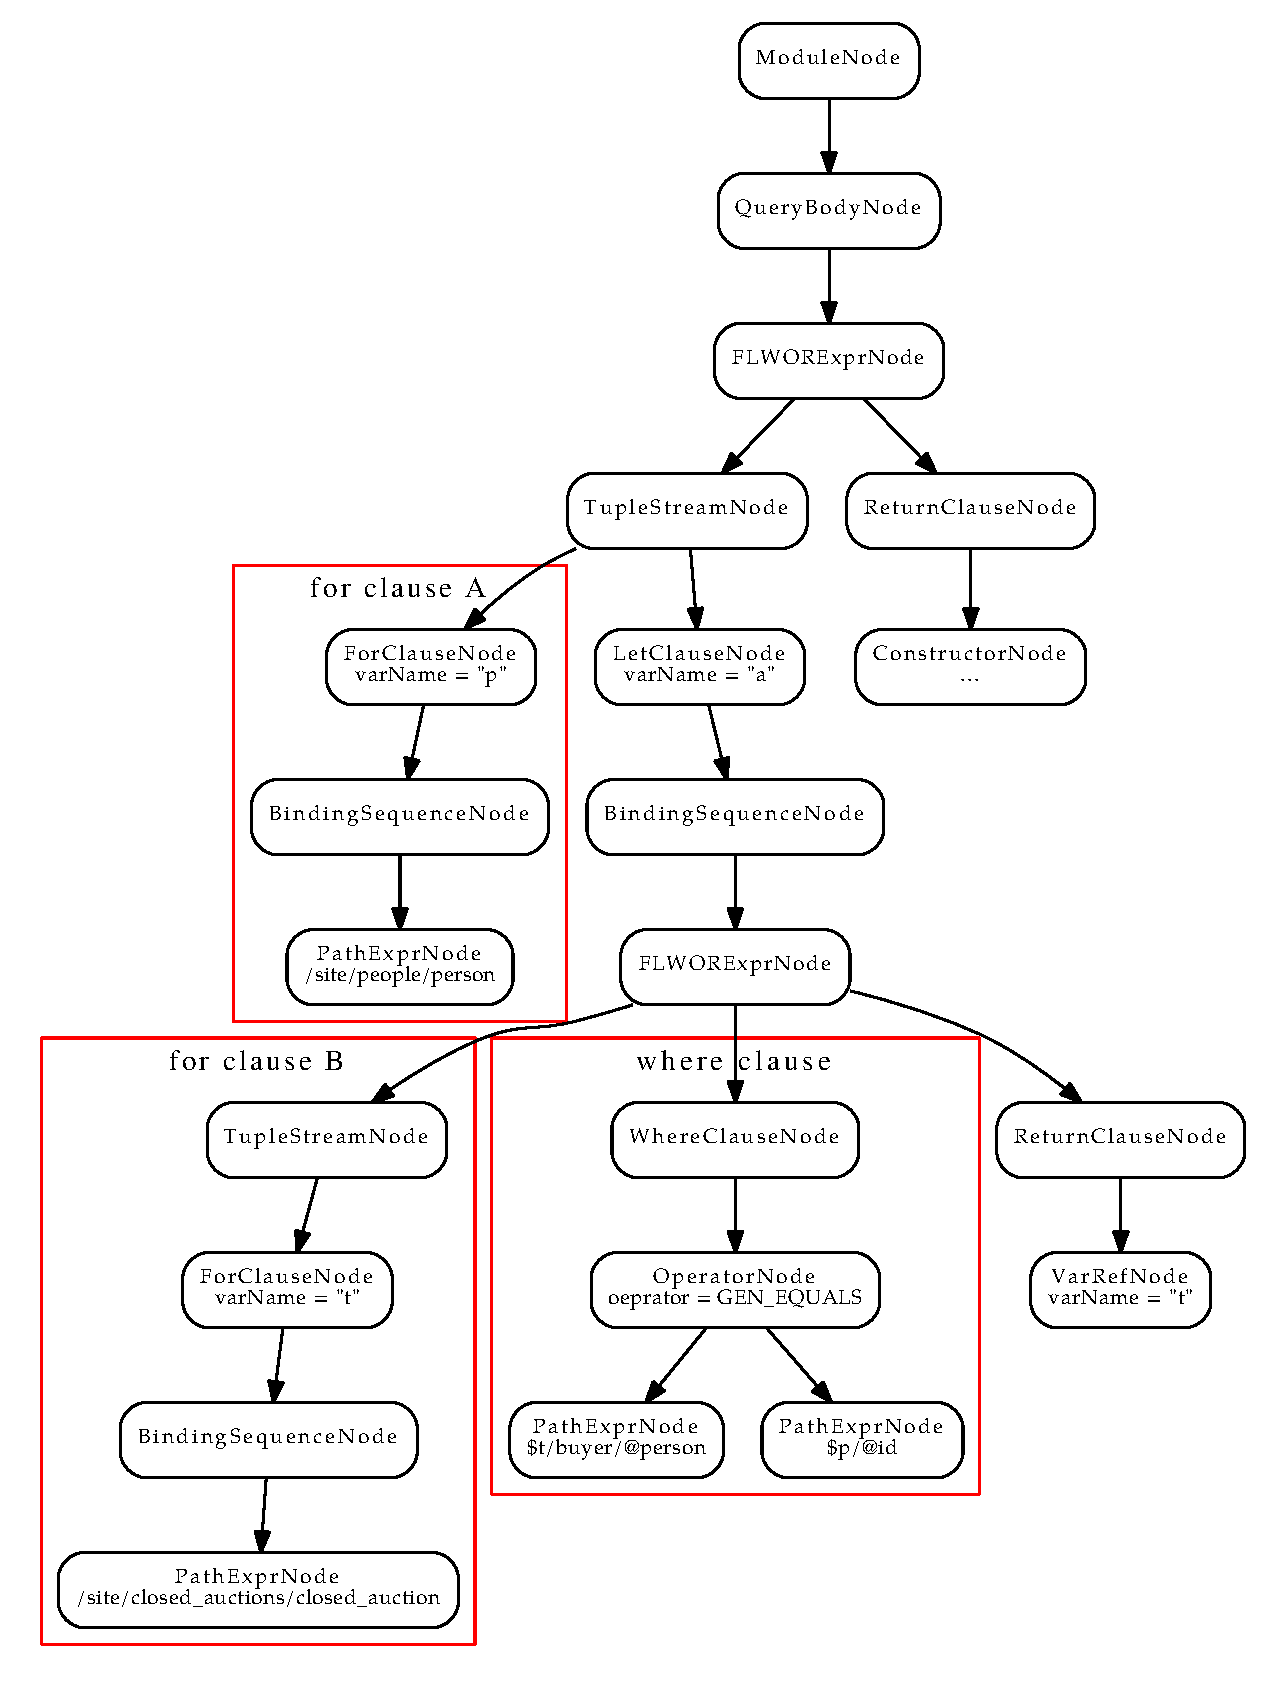
\includegraphics[scale=0.7]{syntax_tree_2.eps}
\end{figure}

Figure \ref{FIG_syntax_tree_2} shows the syntax tree of the query in Listing \ref{listing_sample_query_2}. In this tree, the algorithm founds one occurrence of the join pattern 3. The two for clauses and one where clause which form the occurrence are shown in the red boxes.

The next phase marks this occurrence as (O1) case with weight 0.5 and the following statements are inferred:

\begin{itemize}
\item Key $k = (/site/people/person, \{@id\})$ is satisfied.
\item Foreign key $((/site/closed\_auctions/closed\_auction, \{buyer/@person\}) \rightarrow k)$ is satisfied.
\item Key $(/site/closed\_auctions/closed\_auction, \{buyer/@person\})$ is not satisfied.
\end{itemize}